\documentclass[12pt]{article}

\usepackage[margin=1in]{geometry}
\usepackage{amsmath}
\usepackage{biblatex}
\usepackage{graphicx}
\usepackage{float}
\usepackage{setspace}
\usepackage{fancyhdr}
\usepackage{lastpage}
\usepackage{titlesec}
\usepackage{enumitem}
\usepackage{subfig}
\usepackage{hyperref}
\usepackage{soul}

\pagestyle{fancy}
\renewcommand{\headrulewidth}{0pt}
\renewcommand{\footrulewidth}{0pt}
\fancyhf{}
\lfoot{\scriptsize January 2019}
\cfoot{\scriptsize Brendon Matusch---Improving Particle Classification in WIMP Experiments}
\rfoot{\scriptsize Page~\thepage~of~\pageref{LastPage}}

\setlist[enumerate]{noitemsep, nolistsep}
\setlist[itemize]{noitemsep, nolistsep}

\graphicspath{{./images/}}

\addbibresource{paper.bib}

\titlespacing{\section}{0pt}{0pt}{0pt}
\titlespacing{\subsection}{0pt}{0pt}{0pt}
\titlespacing{\subsubsection}{0pt}{0pt}{0pt}

\setlength{\belowcaptionskip}{-12pt}

\titleformat*{\section}{\large\bfseries}
\titleformat*{\subsection}{\normalsize\bfseries}
\titleformat*{\subsubsection}{\normalsize\bfseries}

\doublespacing

\begin{document}

\begin{center}
    \begin{LARGE}
        Improving Particle Classification in WIMP Dark Matter Detection Experiments Using Neural Networks
    \end{LARGE}

    Brendon Matusch
\end{center}

\section{Introduction}

In all experiments for detection of WIMP dark matter, it is essential to develop a classifier that can distinguish WIMP events from background radiation, in particular alpha particles. Manually developing such a classifier necessitates time-consuming physical modeling.

Machine learning (ML) has the potential to automate this and accelerate experimentation, and also to detect patterns that humans cannot. However, impure calibration data hinders training of models, and unusual detector topologies make data challenging to process.

I worked with two dark matter experiments: the PICO-60 bubble chamber \cite{pico}, and the DEAP-3600 liquid argon scintillator \cite{deap}. In PICO-60, background alpha and WIMP-like neutron calibration datasets are used for training; however, there is an impurity of 10\% alphas in the neutron set, hindering training. In DEAP-3600, the detector format, containing 255 spherically arranged photomultiplier tubes (PMTs), makes data processing challenging.

Previously in PICO-60, a conventional classifier was developed and is thought to be 100\% accurate. However, machine learning is also applicable because it is quicker to develop and re-calibrate. A supervised neural network was used, reaching a mean of 80.2\% accuracy.

In DEAP-3600, in a simulated environment, a conventional classifier removes 99.6\% of alpha background radiation, while also (undesirably) removing 91.0\% of WIMP events.

My objective was to develop novel machine learning algorithms that are more accurate, and I succeeded at this goal! I composed a 26-page research whitepaper \cite{me} about my work on PICO-60, which has been approved by the PICO collaboration and pre-published at \url{https://arxiv.org/abs/1811.11308}.

\ul{Please note that the entire PICO collaboration are listed on the research whitepaper because of their contributions to the original PICO-60 dark matter experiment. They did not contribute to this study; I completed and documented it entirely independently.}

\section{Procedure}

\subsection{PICO-60}

For PICO-60, I developed and compared two sets of classification algorithms:

\begin{enumerate}
    \item I experimented further with supervised learning, exploring the following data formats to learn which was the best-performing solution:
    \begin{itemize}
        \item An 8-band Fourier transform of audio recorded in the bubble chamber. I applied a dense neural network with dropout \cite{dropout} and L2 regularization (which allowed for less overfitting to impure data).
        \item A full-resolution Fourier transform of the audio (all 50,001 data points). I once again applied a dense neural network with the Adam \cite{adam} optimizer.
        \item A raw audio waveform with a very deep 1D convolutional neural network (CNN) inspired by Dai et al \cite{verydeepconvnets}.
        \item Images captured by cameras in the detector. I trained a 2D CNN on these, to learn whether they contain any relevant information.
    \end{itemize}
    \begin{figure}[ht]
        \centering
        \subfloat{\fbox{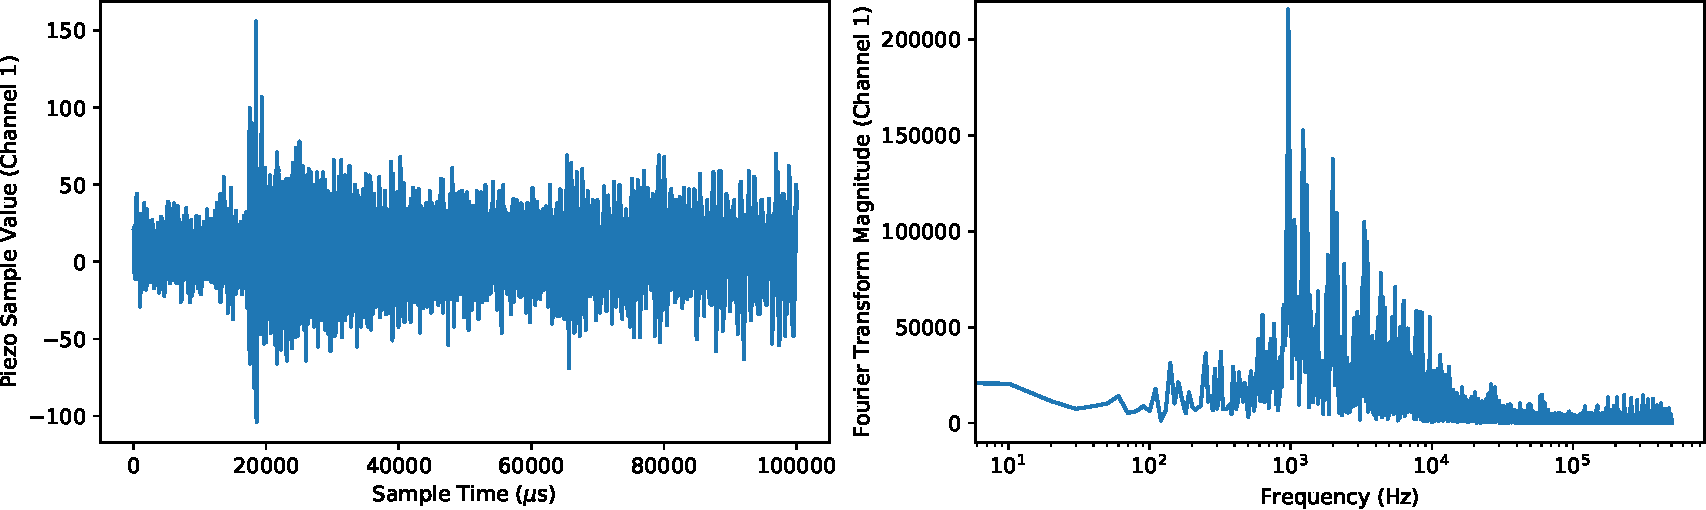
\includegraphics[width=0.9\textwidth]{audio_cropped}}}
        \qquad
        \subfloat{\fbox{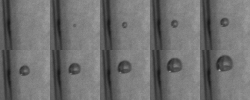
\includegraphics[width=0.45\textwidth]{image_grid}}}
        \caption{Examples of the audio waveform and Fourier transform (above) and the images captured by cameras (below).}
    \end{figure}
    \item To even better handle impurities, I developed two novel semi-supervised learning algorithms. The impure alpha/WIMP-like labels were removed from a large portion of the training data, and my algorithms learned more accurate labels for this data.
    \begin{itemize}
        \item Iterative Cluster Nucleation is inspired by unsupervised clustering algorithms. A neural network is trained on a labeled set, and runs inference on the unlabeled set. Unlabeled examples with predictions closest to 0 or 1 are added to the labeled set; the newly synthesized labels are more accurate than the original labels.
        \item Gravitational Differentiation uses a novel piecewise exponential function to calculate final-layer gradients. Unlabeled examples ``gravitate'' toward more accurate predictions based on the confidence of the neural network's predictions.
    \end{itemize}
\end{enumerate}

\subsection{DEAP-3600}

In DEAP-3600, the key challenge is the aforementioned unusual detector format: a sphere tiled with a hexagonal lattice of PMTs. I approached this problem in three different ways:

\begin{enumerate}
    \item I tried simply inputting photon counts from each PMT into a multi-layer perceptron.
    \item I developed and applied a Mercator-like cylindrical projection, and used a 2D CNN.
    \item I developed an entirely new type of CNN, called a topological CNN. Rather than a 2D image of square pixels, kernels convolve over an arbitrary topology.
\end{enumerate}

\begin{figure}[ht]
    \centering
    \subfloat{\fbox{
\includegraphics[width=0.45\textwidth]{map_projection}}}
    \qquad
    \subfloat{\fbox{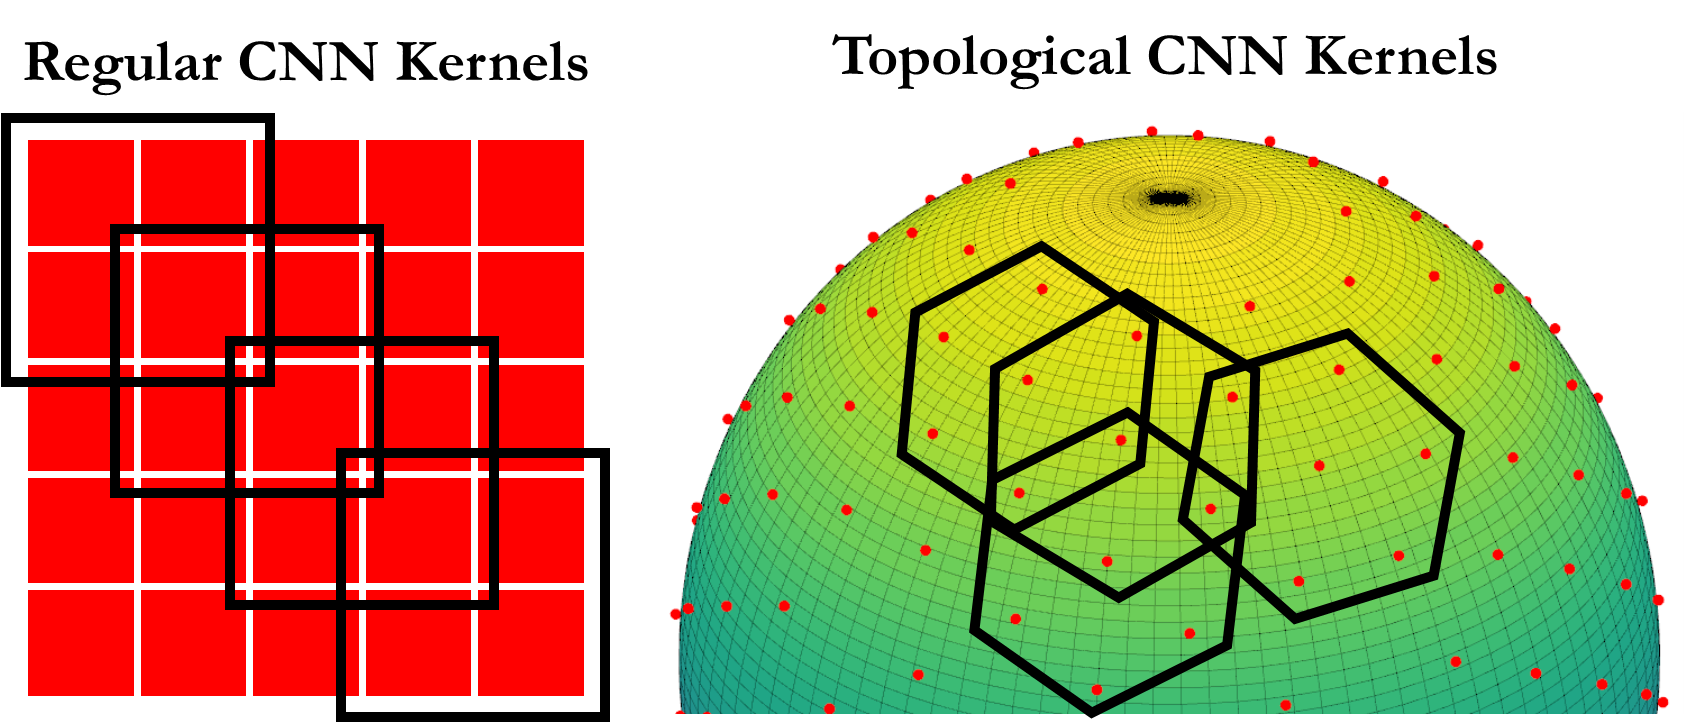
\includegraphics[width=0.45\textwidth]{topological}}}
    \caption{Diagrams of the map projection (left) and topological CNN (right) systems.}
\end{figure}

\subsection{Statistical Practices}

All models were trained on a training set, and a separate randomly selected validation set was used to select the best-performing technique and corresponding hyperparameters (with a grid search). A test set was used to verify the performance of the model ultimately chosen.

\section{Results}

\subsection{PICO-60}

\begin{itemize}
    \item The dense neural network, with banded Fourier transform data, increased validation accuracy to 97.3\% on validation data, up from the previous ML accuracy of 80.2\%.
    \item The full-resolution Fourier transform unexpectedly worsened accuracy to 92.2\%.
    \item The raw waveform with a 1D very deep CNN reached 94.5\% accuracy.
    \item There was no useful information in the image data; only 63.0\% accuracy was achieved.
    \item Iterative cluster nucleation, using banded FT input data, improved accuracy to 99.1\%.
    \item Gravitational differentiation was even more accurate, at 99.7\%.
    \item The best gravitational differentiation configuration was not as accurate on final test data as on validation data, but was much better than supervised learning, at 98.3\%.
\end{itemize}

\begin{figure}[ht]
    \centering
    \fbox{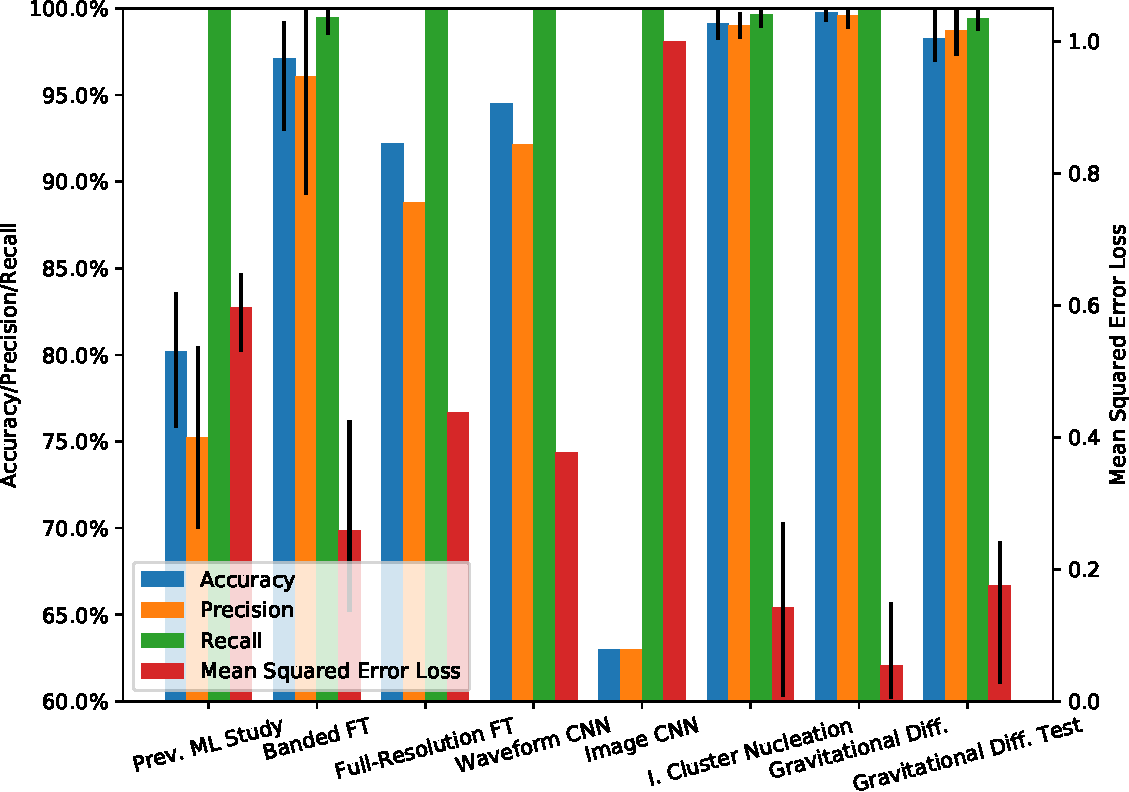
\includegraphics[width=0.95\textwidth]{pico_final_results}}
    \caption{Validation accuracy, precision, recall, and loss for each technique in PICO-60. Error bars represent the 8th and 92nd percentiles.}
\end{figure}

\subsection{DEAP-3600}

The three algorithms I developed were evaluated based on their reduction in the rate of false positives (simulated WIMP events misidentified as neck alphas) compared to the 91.0\% result achieved with a conventional classifier. Only models with at least 99.6\% neck alpha removal (in line with the conventional classifier) were considered.

\begin{itemize}
    \item The dense neural network always produced 100\% false positives (worse than 91.0\%).
    \item The topological CNN produced a false positive rate of 92.6\% (also worse than 91.0\%).
    \item The cylindrical projection method with a 2D CNN improved the false positive rate from 91.0\% to 75.7\% (a 63.0\% reduction)!
\end{itemize}

\begin{figure}[ht]
    \centering
    \fbox{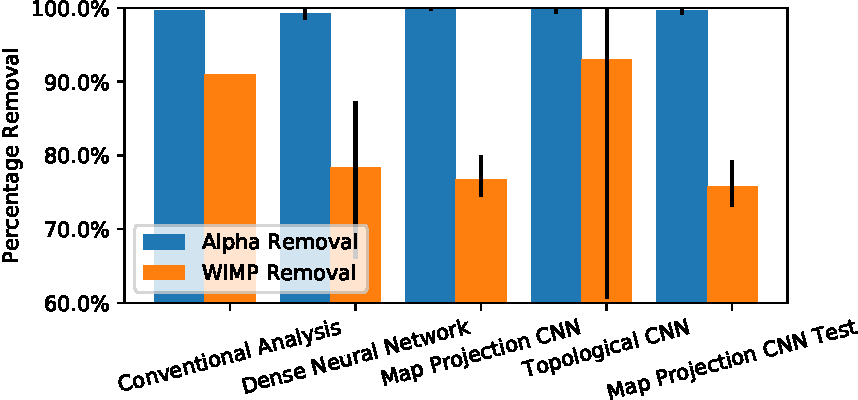
\includegraphics[width=0.6\textwidth]{deap_final_results}}
    \caption{Alpha background and WIMP removal rates for the highest-accuracy hyperparameter configuration of each technique in DEAP-3600.}
\end{figure}

\section{Conclusion}

These results confirm that I achieved my goal. While the conventional classifier in PICO-60 is believed to be perfectly accurate, my semi-supervised learning methods have significantly improved the accuracy that can be obtained quickly and without manual optimization. This should allow physicists working on future iterations of PICO to iterate more quickly, without modifying a conventional classifier whenever some aspect of the experiment changes.

The reduction in the false positive rate for DEAP-3600 provides evidence that machine learning can improve the efficiency of this experiment, possibly reducing the operation time required to collect sufficient evidence for or against the existence of WIMP dark matter.

Fundamentally, the problems I have solved are not specific to PICO-60 and DEAP-3600; they are common across many dark matter detection experiments. Thus, my algorithms are broadly applicable, and demonstrate promise in the field as a whole.

\section{Acknowledgements}

Many thanks to Dr.~Nigel~Smith, Dr.~Ken~Clark, Dr.~Carsten~Krauss, Dr.~Scott~Fallows, Dr.~Eric~V\'azquez-J\'auregui, and Dr.~Pierre~Gorel for introducing me to PICO-60 and DEAP-3600, and generously providing access to data for training.

\singlespacing
\printbibliography
\doublespacing
\pagebreak

\section*{Bibliography}

\begin{itemize}
    \item All programming for this study was done in Python 3 \cite{python}.
    \item Keras \cite{keras}, running on a TensorFlow \cite{tensorflow} backend, was used for all machine learning tasks.
    \item NumPy \cite{numpy} and SciPy \cite{scipy} were used for linear algebra and signal processing.
    \item ROOT \cite{root}, scikit-image \cite{scikit-image}, and scikit-learn \cite{scikit-learn} were used for data loading and storage.
    \item Matplotlib \cite{matplotlib} was used for data visualization.
\end{itemize}

\end{document}